\chapter{PAC Learning}

\section{Priors}

The appendix is quite helpful for bounds used throughout the text. As the
authors state, ``The book of Kearnsand Vazirani (1994) is an excellent
reference dealing with most aspects of PAC-learning and several other
foundational questions in machine learning. Our example
of learning axis-aligned rectangles, also discussed in that reference, is
originally due to Blumer et al. (1989)."

Mohri's course notes will be helpful: \url{https://cs.nyu.edu/~mohri/ml20/}.
Note that the textbook pdf is freely available on his website, too. Familiarity
with data science fundamentals, multivariable calculus, linear algebra, and
algorithmic analysis is assumed for this specific text. Knowledge of convex
optimization (or nonlinear programming) and real analysis would be very useful,
it seems.

I include a ``corrected" and (imo) clearer proof from other authors that do not
assume continuity of distribution under the chapters folder:
\url{http://compbio.fmph.uniba.sk/vyuka/ml/handouts/rectangles_correction.pdf}

For proofs throughout: For implication $p \implies q$, an antecedent (or
hypothesis) $p$ is a sufficient condition for a consequent (a conclusion) $q$
when the truth of $p$ alone implies the truth of $q$; however, $p$ being false
does not always imply that $q$ is also false. A necessary condition is when the
truth of $q$ is guaranteed by the truth of $p$, or we can say that the truth of
$p$ is implied
by the truth of $q$; in other words, $p$ is not possible without $q$. Several
necessary conditions may induce a condition whereas a sufficient condition is
alone enough to produce the said condition. The sufficient term is the part
that immediately follows ``if'' and the necessary term is the part that
immediately
follows the ``then''. Note that these are converses, but the converse may not
always be true. Further reading:
\url{https://philosophy.stackexchange.com/questions/22/what-is-the-difference-between-necessary-and-sufficient},
\url{https://www.kaptest.com/study/lsat/lsat-formal-logic-necessary-vs-sufficient/}

\section{Exercises}

\exercise{2.1}{
	Necessary and sufficient: a concept class $\mathcal{C}$ is efficiently
	PAC-learnable using hypothesis space  $\mathcal{H}$ in the standard PAC
	model
	if and only if it is efficiently PAC-learnable using the hypothesis
	space
	$\mathcal{H} \cup \{h_0, h_1\}$ in the two-oracle PAC model.\\ \\
	Sufficiency: Show that if $\mathcal{H}$ is PAC-learnable in the
	standard,
	one-oracle model then so too is it in the variant.\\

	Since  $\mathcal{C}$ is efficiently PAC-learnable using  $\mathcal{H}$,
	there exists an algorithm $\mathcal{A}$ and a polynomial $p$ such that
	for any
	distribution $\mathcal{D}$ and any target concept $c \in \mathcal{C}$,
	if
	$\mathcal{A}$ is given a sample of size $m \geq p(1/\epsilon,
		1/\delta, n, size(c))$ drawn
	from $\mathcal{D}$, it outputs a hypothesis $h$ from $\mathcal{H}$ such
	that
	with probability at least $1 - \delta$, the error of $h$ on
	$\mathcal{D}$ is at
	most $\epsilon$. Assume a distribution $\mathcal{D}$ on $\mathcal{X}
		\times \{-1, +1\}$.
	The learner's goal is to output a hypothesis with such probability over
	the
	choice of two training sets (in the stochastic scenario where the
	output label
	is a probabilistic function of the input, thus does not guarantee
	unique
	labels)
	and requires both $\mathbb{P}[R(h)_{x \sim \mathcal{D}_{+}} \leq
			\epsilon] \geq 1 - \delta$ and $\mathbb{P}[R(h)_{x
					\sim \mathcal{D}_{-}} \leq
			\epsilon] \geq 1 - \delta$. By the law of total
	proability for
	the error rate (or risk),
	\begin{flalign*}
		R(h)_{\mathcal{D}} & = \underset{x \sim
			\mathcal{D}}{\mathbb{E}}[\mathbb{1}_{h(x) \neq
				c(x)}] = \sum_{x \in
			\mathcal{D}} x \mathbb{P}[\mathbb{1}_{h(x)
				\neq c(x)}] =	     \underset{x \sim
			\mathcal{D}}{\mathbb{P}}[h(x) \neq
			c(x)]
		\\
		                   &
		=\mathcal{D}(\mathcal{X}^+)(R(h)_{\mathcal{D}_{+}})+\mathcal{D}(\mathcal{X}^-)(R(h)_{\mathcal{D}_{-}})
	\end{flalign*}
	Now for a weighted sampling method from the negative and positive
	instance distributions we can say $\epsilon_{\mathcal{D}} =
		\mathbb{P}[\mathcal{D}^+](\alpha
		\epsilon)_{\mathcal{D}^+}+\mathbb{P}[\mathcal{D}^-](\beta
		\epsilon)_{\mathcal{D}^-} =  \epsilon
		\underbrace{(\mathbb{P}[\mathcal{D}^+](\alpha -
			\beta)+\beta)}_{\leq 1}$ for some constants $0 \leq
		\alpha, \beta \leq 1$.
	Note that $\alpha = \beta = 0 \implies \epsilon = 0$,
	which means you're demanding that the learned hypothesis
	perfectly match the true target function,
	which can lead to overfitting and complex hypotheses that are
	computationally expensive to work with (recall $\epsilon > 0$
	by definition). Conversely, by setting
	$ \epsilon  =1$, you're ok accepting any hypothesis without
	regard to its performance.
	Thus, select an
	appropriate $\delta$ and, for simplicity, set
	$\mathbb{P}[\mathcal{D}^+] =
		\frac{1}{2}$, to get
	\begin{flalign*}
		\mathbb{P}[R(h)_\mathcal{D} \leq \frac{\alpha \epsilon}{2}]
		           &
		\geq 1 - \delta
		\\
		\frac{1}{2}(\mathbb{P}[R(h)_{\mathcal{D}_{+}} \leq \alpha
			\epsilon]+\mathbb{P}[R(h)_{\mathcal{D}_{-}} \leq \alpha
		\epsilon]) & \geq 1 -
		\delta
	\end{flalign*}
	If we set $\alpha = 1$ for this case we then see that by selecting
	$\mathbb{P}[R(h)_\mathcal{D} \leq \frac{\epsilon}{2}]$ with an
	appropriate
	confidence interval, we must have that both
	$\mathbb{P}[R(h)_{\mathcal{D}_{-}}
			\leq \epsilon], \mathbb{P}[R(h)_{\mathcal{D}_{+}} \leq
			\epsilon] \geq 1 -
		\delta$.  We immediately
	notice that a biased dataset would then require us to make considerable
	adjustments to the overall error rate, as $\mathcal{D}^+$ will shift
	the weight of distribution of samples. Another thing to note is that by
	setting $\alpha$ or $\beta$ to 0, we're essentially requiring
	that the hypothesis have zero error on positive (or negative)
	instances (perhaps requiring an absurdly complex hypothesis to do so).
	This
	transforms the problem into a rather stringent one-oracle PAC model
	focused
	solely
	on the positive (or negative) class which is not sensitive to noise.
	The PAC framework is designed to find a balance between minimizing
	errors on
	both classes while accounting for uncertainties in real-world data;
	this decoupled mode
	tells the learner to query the oracle for
	instances of one class while imposing stringent error requirements on
	the other
	class. \\ \\

	Necessary: Show that if $\mathcal{H}$ is PAC-learnable in the
	two-oracle variant, it is also PAC-learnable in the standard model.\\\\

	We now can assume that $\mathcal{C}$ is efficiently PAC-learnable in
	the two-oracle PAC model so there
	exists an algorithm $\mathcal{A}$ such that for $c \in \mathcal{C}$,
	$\epsilon, \delta >0$, there are $m^+$ and $m^-$
	in $p(1/\epsilon, 1/\delta, size(c))$, such that if we draw at least
	this
	number of negative and positive instances with confidence of at least
	$1 - \delta$,
	the
	hypothesis $h$ output by the learner satisfies:
	\begin{flalign*}
		R(h)_{\mathcal{D}^{+,-}}             & \leq \epsilon \\
		\mathbb{P}[R(h)_{\mathcal{D}^{+,-}}] & \leq
		\mathbb{P}[\epsilon] = \epsilon
	\end{flalign*}
	So, given sufficient numbers of negative and positive examples, we can
	generate a hypothesis $h$ such that it has low errors on both negative
	and
	positive instances.
	If we draw too few examples, the conclusions about the hypothesis's
	performance might not hold true for the entire distribution
	(generalize); to
	bridge the gap between the variant and standard model it is then best
	to take $m \geq \max\{m^+, m^-\}$ and, drawing such with polynomial
	conditions above and using the union bound and total probability,
	\begin{flalign*}
		\mathbb{P}[R(h)_{\mathcal{D}}] & \leq
		\mathbb{P}[\mathcal{D}^+]\mathbb{P}(R(h)_{\mathcal{D}_{+}})+
		\mathbb{P}[\mathcal{D}^-]\mathbb{P}(R(h)_{\mathcal{D}_{-}})=
		\mathbb{P}[R(h)_{\mathcal{D}}|c(x) \neq -1]\mathbb{P}[c(x) \neq -1] +
		\mathbb{P}[R(h)_{\mathcal{D}}|c(x) \neq 1]\mathbb{P}[c(x) \neq 1]                              \\
		                               & \leq \epsilon(\mathbb{P}[c(x) \neq -1] + \mathbb{P}[c(x) \neq
		1]) \leq \epsilon                                                                              \\
	\end{flalign*}
	Let $X$ be the total number of positive examples obtained from drawing
	$m$ examples, with probability of a positive example of $\epsilon$ as shown
	above.
	\begin{flalign*}
		\mathbb{P}\Bigg[\frac{X}{m} \geq (1-\gamma) \epsilon  \Bigg]
		\leq e^{-\frac{m \epsilon \gamma^2}{3}} \leq \delta
	\end{flalign*}
	Setting (a rather lax) $\gamma = \frac{1}{2}$, required that $\gamma
		\in [0, 1/\epsilon - 1]$, to match conditions above and needing $m^+ =
		m(1-\gamma)\epsilon = \frac{m \epsilon}{2}$,
	\begin{flalign*}
		\mathbb{P}\Bigg[X \geq m^+  \Bigg] & \leq e^{-\frac{m^+}{6}}
		\leq \frac{\delta}{2}                                        \\
	\end{flalign*}
	Since we want to include the minimum number of positive instances, we
	set the latter expression to an appropriate bound $\delta/2$ (from above, we
	saw that using an even split weight between negative and positive examples with
	overall $\epsilon/2$ as we set here, so can use 2(1-$(\delta/2)) > 1-\delta$)
	and subsitute back to get an expression of $m \geq \min
		\{\frac{2m^+}{\epsilon}, \frac{12}{\epsilon}\log(2/(\delta))\}$. A similar
	procedure is done with the negative case to arrive at $m \geq \min
		\{\frac{2m^+}{\epsilon}, \frac{2m^-}{\epsilon},
		\frac{12}{\epsilon}\log(2/(\delta))\}$ for a balanced dataset.
}

Good learners will learn with high proability and close approximation to the
target concept. With high probability, we find a hypothesis that will have low
error (approximately correct), requiring parameters $\epsilon, \delta > 0$.
Thus, with probability of at least $1-\delta$, the algorithm learns the concept
with error at most $\epsilon$. The $\epsilon$ is the upper bound on the
accuracy ($1-\epsilon$). We use $\delta$ to bound the probability of failure in
achieving the set accuracy (a bad event) and thus want a hypothesis to be
approximately correct with confidence $1-\delta$.\par
Yessir

\centering
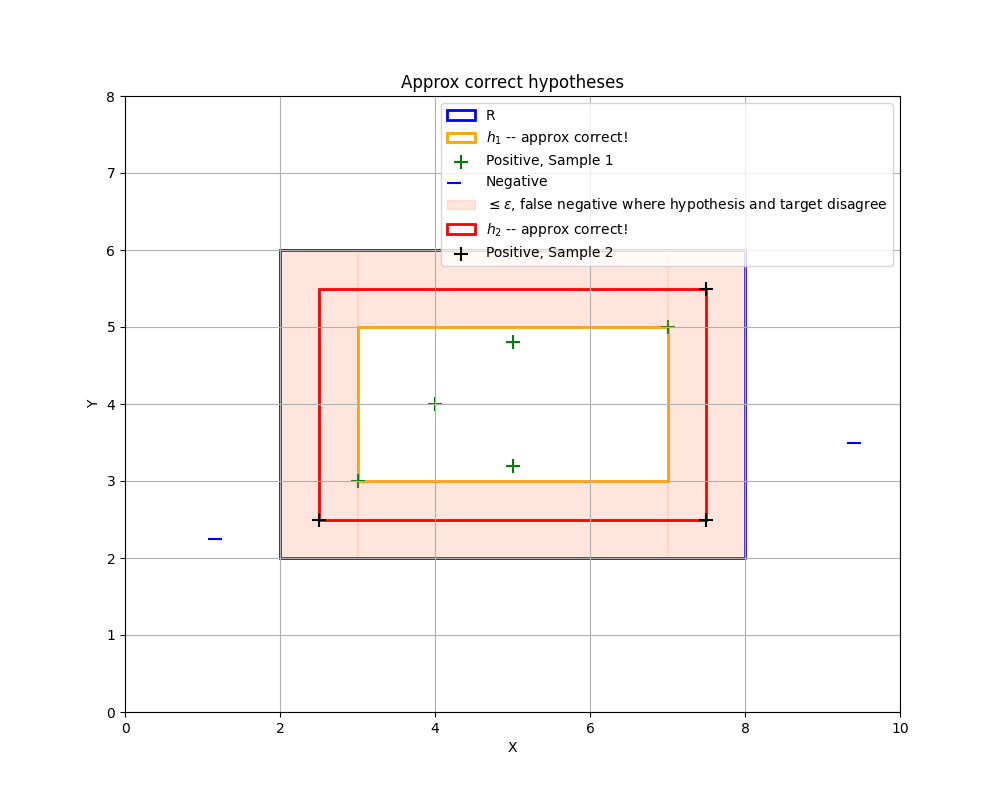
\includegraphics[width=0.8\textwidth]{./chapters/goodPAC.png} 
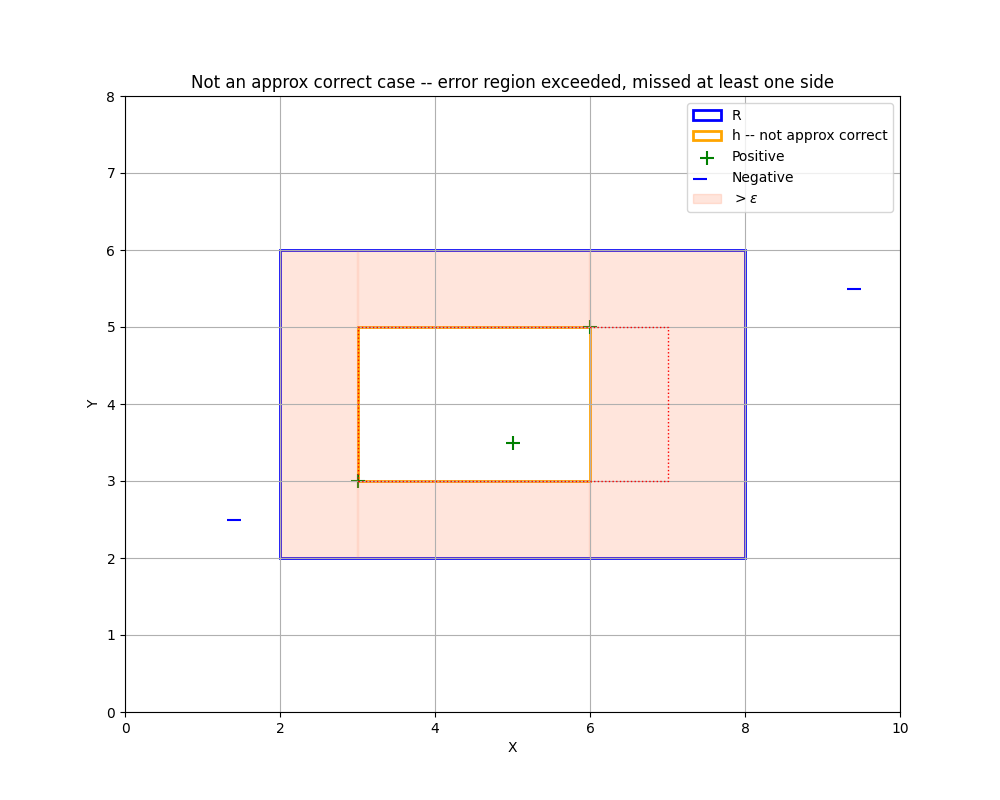
\includegraphics[width=0.8\textwidth]{./chapters/badPAC.png} 
